\chapter*{Choices in Technologies    \chapter{Actors}
\label{ch:actors}

Actors specify a role played by a user or a system for the purposes of a clearer definition.
In this chapter, we will outline the actors in our system.

\begin{landscape}
	\topskip0pt
	\vspace*{\fill}
	\section{Big Picture}
	\begin{figure}[H]
		\begin{center}
			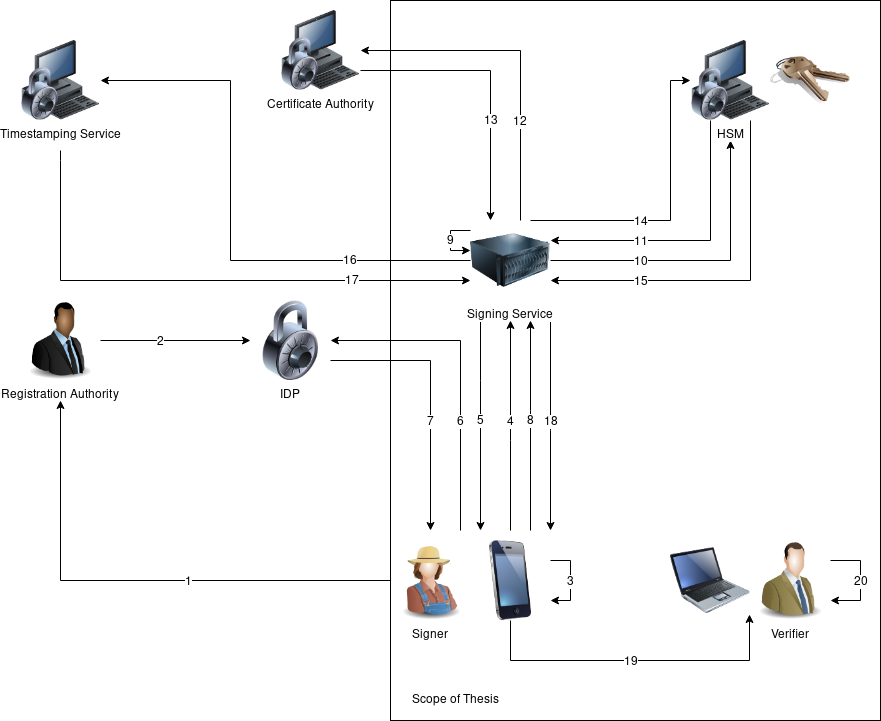
\includegraphics[scale=0.6]{images/BigPicture.png}
			\caption{Big Picture}
			\label{fig:bigpicture}
		\end{center}
	\end{figure}
	\vspace*{\fill}
\end{landscape}

\subsubsection{Steps}
\begin{enumerate}
	\item Registration of identity with RA (Authenticator)
	\item Propagate identity to IDP (Identifier)
	\item Generate document hash
	\item Send hash to signing service
	\item Receive OIDC redirect to IDP
	\item Login to IDP
	\item Receive ID token
	\item Send ID token to signing service
	\item Verify ID token
	\item Request signing key CSR from HSM
	\item Receive CSR
	\item Send CSR to CA
	\item Receive signed Certificate
	\item Request signature from HSM
	\item Receive signature
	\item Request timestamp from TSS
	\item Receive timestamp
	\item Send signature to signer
	\item Send document and signature to Verifier/Receiver
	\item Verify document and signature
\end{enumerate}


\section{The Signer}
\label{sec:actorsigner}
The Signer is the person who wishes to have the signing server sign a document in their name.
For example, a medical professional issuing a prescription for medication to a patient.

\section{The Verifier}
\label{sec:actorverifier}
The Verifier is the person who wishes to verify the integrity and authorship of a document.
For example, the pharmacist whom the patient gives the prescription to (as previously authored and signed by The Signer as specified in section~\ref{sec:actorsigner}) in order to purchase the medication prescribed by the medical professional.

\section{The Authenticator}
\label{sec:actorauthenticator}
The Authenticator is the system who authenticates The Signer as specified in section~\ref{sec:actorsigner}.
In \gls{NIST} terminology~\cite{nistdigitalidentityguidelines}, this is the entity establishing the \gls{IAL}.
In order for The Authenticator to be able to authenticate The Signer,
they must have been registered with The Authenticator by The Identifier as specified in section~\ref{sec:authoridentifier}.

\section{The Identifier}
\label{sec:authoridentifier}
The Identifier is the system or person who asserts the identity of The Signer.
In order for the signing service to issue qualified signatures as defined by relevant Swiss legislation~\cite{zertes} and Swiss Federal Council regulations~\cite{vzertes},
the identity must be proven in-person using a government-issued photographic identification document such as a passport.

\section{The Signing Service}
\label{sec:signingservice}
The Signing Service is the system who actually creates the signatures on behalf of the user.
It generates the signing keys and requests the \gls{CA}~\ref{sec:ca} to sign them.

\section{The Certificate Authority}
\label{sec:ca}
The \gls{CA} is the system who signs the signing keys generated by the Signing Service~\ref{sec:signingservice}.
}
\label{ch:techchoices}
In this chapter, we outline the technologies we choose, and the reasoning for choosing them.

\section{Backend}
\label{sec:techbackend}
It is implemented using the Play Framework~\cite{playframework} and the Scala~\cite{scalalang} programming language.
TODO explain why.

\section{Frontend}
\label{sec:techfrontend}

Given that the frontend must support the three desktop operating systems Microsoft Windows, GNU/Linux as well as Apple MacOS,
the technological choices available to us are limited.
On the desktop, we could use the \gls{JVM} platform and the JavaFX \gls{GUI} library, whereas on the phones
we could use Flutter~\cite{flutterframework}.
However, developing three applications on five platforms using two new-to-us frameworks and programming languages
would take a lot more time and resources than what is available to us in the scope of this thesis.

In order to reduce complexity we decide to implement the frontend as a web application, capable of running
in any modern web browser regardless of platform, be it mobile or desktop.
We're not happy about this, as we would much rather use mature, strongly-typed and well-designed languages and frameworks,
but we're forced to make this compromise in order to meet our objectives in the time available.
In order to reduce the pain, we will use TypeScript, which is a strongly typed superset of JavaScript~\cite{loltypes}.

\subsection{Client-Side File Hashing in the Web Browser}
\label{subsec:browserhashing}
This decision presents us with a challenge: hashing the files to be signed client-side in the web browser itself.
If we had implemented "proper" client applications this would've been easy, but in a web browser and using its
JavaScript language not so much: they weren't designed with file I/O and CPU-intensive cryptographic functions in mind.
The easiest solution would be to upload the files to be signed to the server and hash them there,
but this would be a clear violation of the least-information principle (the server doesn't need the file, only the hash)
and a breach of user privacy.
Another solution would be to ask the user to enter the file hashes instead of selecting files,
but this would be very user-unfriendly and probably downright impossible for many people.

It is clear we must find a way to hash files in the web browser itself.
In order to achieve this we have found the following options:

\begin{enumerate}
    \item Using the browser-implemented \texttt{SubtleCrypto}~\cite{subtlecrypto} \gls{API}
    \item Using the \texttt{CryptoJS}~\cite{cryptojs} JavaScript implementation
    \item Using a \gls{WASM}-based implementation
\end{enumerate}

Each of these options comes with a number of advantages and disadvantages, as discussed in more detail in the following sections.

\subsubsection{Using SubtleCrypto}
\label{subsubsec:subtlecrypto}
The \texttt{SubtleCrypto} class offers the \texttt{digest(algorithm, data)} method~\cite{subtlecrypto}, which can be used to
calculate \gls{SHA-256} checksums.
The advantage of using this implementation is that it is available in all modern browsers\footnote{Where modern browsers means Mozilla Firefox, Google Chrome/Chromium, and Microsoft Edge},
and since it's executed with native code, being able to take advantage of \gls{AVX2} instructions, instead of JavaScript it should be quite fast.
There's a major drawback though: hashing a large amount of data progressively is not supported, the data has to be
passed to the function en bloc, as seen in listing~\ref{lst:subtlecrypto}.

\begin{lstlisting}[caption={Using SubtleCrypto for calculating SHA-256 checksums}, captionpos=b, language=JavaScript, label={lst:subtlecrypto}]
crypto.subtle.digest("SHA-256", data).then(hash => {
    console.log(
        // convert ArrayBuffer to hex string
        Array.from(new Uint8Array(hash)).map(
            b => b.toString(16).padStart(2, '0')
        ).join('')
    );
});
\end{lstlisting}
Our testing showed that selecting files larger than 200MB crashes Firefox tabs when trying to read their contents
into memory before we could pass it to the \texttt{digest} function.
If we assume the users will only ever select small files this should not pose a problem, but unfortunately it's not safe to assume this.

\subsubsection{Using CryptoJS}
\label{subsubsec:cryptojs}
\texttt{CryptoJS} does not have the limitation of \texttt{SubtleCrypto} and supports progressive hashing\footnote{
By progressive hashing we mean the ability to pass to the hash function the data piece by piece in order to avoid holding all of it in memory at once.},
as seen in listing~\ref{lst:cryptojsprogressive}.

\begin{lstlisting}[caption={Progressive SHA-256 hashing using CryptoJS},captionpos=b,language=JavaScript,label={lst:cryptojsprogressive}]
const sha256 = CryptoJS.algo.SHA256.create();

sha256.update("Message Part 1");
sha256.update("Message Part 2");
sha256.update("Message Part 3");

const hash = sha256.finalize();
\end{lstlisting}

The advantage of using \texttt{CryptoJS} over \texttt{SubtleCrypto} is, as mentioned, the ability to hash piece-wise.
The disadvantage is that we need to load a third-party JavaScript library, using built-in functionality would be preferable.
And since JavaScript is an interpreted language, using it to calculate the checksums would presumably result in significantly lower performance.


\subsubsection{Using a WASM-based implementation}
\label{subsubsec:wasmhashing}
\gls{WASM} provides a low-level virtual machine running machine-independent binary code, comparable to the \gls{JVM} or the \gls{CLR}, albeit much simpler and much less sophisticated.
By using this virtual machine we should be able to, in theory, run code at near-native speed written in a statically-typed, compiled language such as Rust, C++ or Go.
We expect significant performance gains over a JavaScript-based implementation.
While developing the \gls{WASM}-based hashing program, we encountered some interesting challenges, as described in the following paragraphs.

\paragraph{CORS Policy} While JavaScript can be executed simply by pointing the browser at a local \gls{HTML} file, the same doesn't work for \gls{WASM}.
The browser's security policy forbids it due to its \gls{CORS} rule~\cite{cors}.
We solved this by starting the \gls{HTTP} server built in to Go's standard library and having the browser load the \gls{WASM} binary through \gls{HTTP}.
The code is in appendix~\ref{chap:appendix_golangwebserver}.

\paragraph{JavaScript/WASM Compatibility} The Golang project conveniently provides a file containing the necessary boilerplate code to load, start and interact with \gls{WASM} programmes called \texttt{wasm\_exec.js}.
But there's a catch: for each version of Go, the version of the accompanying \texttt{wasm\_exec.js} file used must match precisely.
If it doesn't, the code will crash with a segmentation fault.
It took us quite some time to figure out why the code we'd written only a few days prior would segfault now with no changes made to it.

\paragraph{Passing data} Functions written in Go intended to be used from the JavaScript side of things need to have a very specific signature.
As can be seen in listing~\ref{lst:funcsignaturewasm}, there is no typing: all arguments passed to the function are of type \texttt{js.Value} and the return value must be of type \texttt{interface\{\}}\footnote{This is Go's equivalent of Java's \texttt{Object}, it could be anything.}.
This posed us with the challenge of detecting the types and casting the data passed accordingly.

\begin{lstlisting}[caption={Golang WASM function signature}, captionpos=b, language=Go, label={lst:funcsignaturewasm}]
    func f(this js.Value, arg js.Value) interface{} {}
\end{lstlisting}

We've worked on this for hours, producing ugly reflection-based hacks, until we decided to just agree on the types of the arguments and return values beforehand despite the open function signature.
Now all that's needed is a little boilerplate to convert a JavaScript \texttt{Uint8Array} to a Golang \texttt{[]byte}, as seen in listing~\ref{lst:jscastingtogo}.

\begin{lstlisting}[caption={Uint8Array to {[]}byte}, captionpos=b, language=Go, label={lst:jscastingtogo}, captionpos=b]
func progressiveHash(this js.Value, in []js.Value) interface{} {
    array := in[0]
    buf := make([]byte, array.Get("length").Int())
    js.CopyBytesToGo(buf, array)
    return this
}
\end{lstlisting}

\paragraph{Goroutines} Go features its own concurrency primitive called Goroutines.
From a programmers' perspective, they can be used like threads, but they carry much less overhead.
Communication between goroutines is achieved by using so-called channels, which on a high level are comparable to queues.
Unfortunately, the \gls{WASM} specification wasn't drafted with this kind of concurrency in mind.
Go is forced to unwind and restore the call stack when switching between goroutines, which is very expensive~\cite{lolnogoroutines}.
We rewrote the Go programme to work without them, and we've seen a small performance improvement, as seen in figure~\ref{fig:hashingperformance}.

\paragraph{Rust based WASM}
As the Go implementation also includes the Go runtime, which makes the wasm file much larger, and starts a program that
will run continuously in the background it isn't the optimal choice for creating a WebAssembly implementation.
As neither of us knows any other choice of the languages that compile to WebAssembly well, we first excluded them.
However with the drawbacks of the Go based implementation we decided to try also implement a Rust based version to see
how they compare both in performance and ease of development.


\subsection{Performance Comparison}
\label{subsec:perfcomphashing}
No one likes waiting for slow software to do its work, and neither do we.
This is why we decided to compare the performance of the aforementioned options in a simple test:
we measure the time it takes for the browser to calculate the checksum of 1GB of random data using the three aforementioned methods.
The code used for each example is in appendix TODO add test code and link here.
The tests were run on Debian 10 using Firefox 69 on an Intel i7-8550U.
The results can be seen in figure~\ref{fig:hashingperformance}.
As expected, the in-browser implementation is the fastest by far, followed by the \gls{WASM}-based implementation.
JavaScript is so slow it's not even competing.
In order to have a baseline reference we compare the hashing speeds to the \texttt{openssl} command-line programme.

\begin{figure}
    \begin{center}
        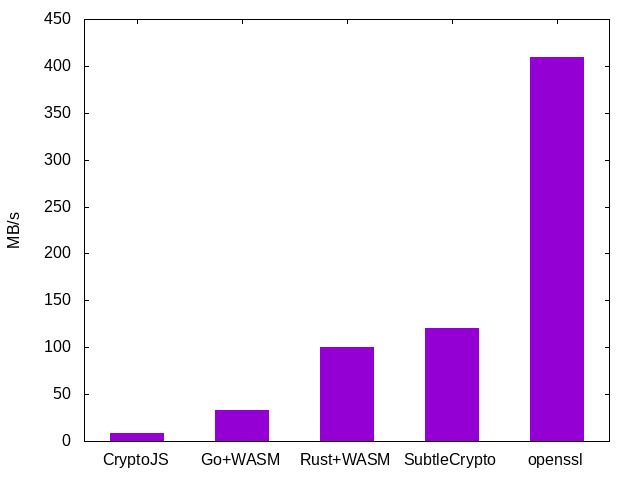
\includegraphics[width=0.7\linewidth]{images/hashingperformance.png}
        \caption{Hashing speed in MB/s (higher is better). Please note that the scale is logarithmic.}
        \label{fig:hashingperformance}
    \end{center}
\end{figure}


\subsection{Deciding On The In-Browser Hashing Implementation}
\label{subsec:deciding-on-the-in-browser-hashing-implementation}
It is clear from figure~\ref{fig:hashingperformance} that \texttt{SubtleCrypto} is significantly faster than the other options we tried.
Unfortunately, since it doesn't support piece-wise hashing we're forced to pick the next-fastest option, the \gls{WASM}-based implementation.













